\documentclass[conference]{IEEEtran}

%% ------ Essential Packages -------------------------------------
\usepackage{cite}
\usepackage{amsmath,amssymb,amsfonts}
\usepackage{algorithmic}
\usepackage{algorithm}
\usepackage{textcomp}
\usepackage{xcolor}
\usepackage{booktabs}
\usepackage{multirow}
\usepackage{url}
\usepackage{pgfplots}
\pgfplotsset{compat=1.18}
\usepackage{tikz}
\usetikzlibrary{arrows.meta, positioning, shapes.geometric, fit, backgrounds, patterns}

\def\BibTeX{{\rm B\kern-.05em{\sc i\kern-.025em b}\kern-.08em
    T\kern-.1667em\lower.7ex\hbox{E}\kern-.125emX}}

\begin{document}

%% ============================================================
%%  TITLE AND AUTHORS
%% ============================================================
\title{Privacy-Preserving Federated Intrusion Detection for\\
Internet of Vehicles Using Single-Key CKKS\\
Homomorphic Encryption and ChebyshevKAN}

\author{
  \IEEEauthorblockN{Author 1}
  \IEEEauthorblockA{\textit{Department Name}\\
  Institution Name\\
  City, Country}
  \and
  \IEEEauthorblockN{Author 2}
  \IEEEauthorblockA{\textit{Department Name}\\
  Institution Name\\
  City, Country}
}

\maketitle

%% ============================================================
%%  ABSTRACT
%% ============================================================
\begin{abstract}
Modern vehicular networks face escalating cyber threats, including
Controller Area Network (CAN) bus injection attacks and Vehicle-to-Everything
(V2X) misbehaviour. Federated Learning (FL) enables collaborative intrusion
detection without sharing raw vehicle telemetry, yet the aggregation server
remains an honest-but-curious adversary capable of inverting individual
model updates to reconstruct sensitive driving data. This paper proposes a
privacy-preserving federated Intrusion Detection System (IDS) for the Internet
of Vehicles (IoV) that combines Single-Key Cheon--Kim--Kim--Song (CKKS)
Homomorphic Encryption (HE) with a novel \emph{ChebyshevKAN} neural network
classifier. The CKKS scheme ($N{=}8192$, 128-bit Ring-LWE security, $2^{40}$
fixed-point scale) packs 4,096 encrypted real-valued parameters per ciphertext,
enabling the RSU server to aggregate 44,164-parameter model updates entirely
within the encrypted domain. By relying purely on CKKS for payload confidentiality,
we remove traditional AES/ECDH transport overhead, streamlining V2X communications.
Extensive experiments on four heterogeneous IoV datasets---Car-Hacking (CAN),
IEEE VTC-CAN, CICIDS-2017, and VeReMi---under a non-IID Dirichlet partition
($\alpha{=}0.3$) demonstrate that CKKS encryption introduces a maximum accuracy
degradation of only $0.01$ percentage points (pp) relative to plaintext federated
averaging, with a per-client ciphertext overhead of ${\approx}3.6$ MB and $1.76$ s
per aggregation round. The system guarantees that individual client updates remain
private throughout training, verified by a runtime audit asserting zero plaintext
leakages.
\end{abstract}

\begin{IEEEkeywords}
Internet of Vehicles, Federated Learning, Homomorphic Encryption, CKKS,
Intrusion Detection, CAN Bus, ChebyshevKAN, Privacy-Preserving Machine
Learning, Non-IID
\end{IEEEkeywords}

%% ============================================================
%%  I. INTRODUCTION
%% ============================================================
\section{Introduction}

Modern vehicles are complex distributed computing networks integrating over
100 Electronic Control Units (ECUs) interconnected through internal
Controller Area Network (CAN) buses and external V2X radio links. This
extended attack surface has made modern connected vehicles vulnerable to
severe cyber exploits, including remote CAN frame injections that override
critical drive-by-wire subsystems such as braking, transmission, and steering.

\textbf{Collaborative IDS and the Privacy Dilemma.}
No single vehicle observes the comprehensive spectrum of vehicular intrusion
vectors: one vehicle travelling on an urban arterial may experience DoS flooding,
while another at a junction encounters malicious RPM spoofing. While pooling
raw CAN frame logs to a centralized server would train an intrusion detector
with broader coverage, CAN logs inherently encode private driver habits,
location trajectories, and vehicle identifiers that cannot leave the vehicle.

Federated Learning (FL) solves the raw-data exposure dilemma by training
models locally on private vehicle shards and communicating only parameter
updates. However, sharing local model gradients introduces an acute secondary
vulnerability: an honest-but-curious Road-Side Unit (RSU) or aggregation server
can employ gradient inversion techniques to reconstruct sensitive training
samples from individual updates.

\textbf{Homomorphic Encryption.}
Fully Homomorphic Encryption (FHE) enables mathematical computations
directly on encrypted ciphertexts. The Cheon--Kim--Kim--Song (CKKS) scheme is
ideally matched for neural network federated learning: it natively supports
approximate floating-point vector arithmetic and offers Single-Instruction
Multiple-Data (SIMD) packing, encoding thousands of parameters into a single
ring ciphertext.

\textbf{Byzantine Robustness in the Encrypted Domain.}
Securing the aggregation server against gradient inspection introduces a
countervailing challenge: conventional Byzantine-robust aggregation algorithms,
such as Multi-Krum and TOPSIS (utilized in our Generation-1 design), require
pairwise Euclidean distance computations over plaintext updates and are
structurally incompatible with FHE. To solve this, we adopt the FheFL
homomorphic non-poisoning-rate filter, evaluating distance metrics relative
to the public global model entirely in the encrypted domain.

%% ============================================================
%%  II. RELATED WORK
%% ============================================================
\section{Related Work}

\textbf{Federated Vehicular IDS.}
Prior collaborative IDS models for IoV rely predominantly on standard
Federated Averaging (FedAvg), transmitting unprotected gradients to an edge
server. Such configurations remain vulnerable to gradient reconstruction
attacks and model poisoning.

\textbf{Homomorphic Encryption in FL.}
Integer-based homomorphic schemes such as Paillier and BFV either mandate
costly fixed-point scalar encodings or restrict SIMD parallelism. CKKS natively
maps floating-point parameters into polynomial rings over cyclotomic fields,
enabling efficient linear vector combinations. FheFL introduced homomorphic
weighting for privacy-preserving federated aggregation, providing the
theoretical framework for our encrypted distance computations.

\textbf{Kolmogorov--Arnold Networks (KANs).}
Traditional Multi-Layer Perceptrons (MLPs) place fixed non-linear activations
on nodes. In contrast, KANs position learnable univariate spline functions
on network edges. While B-spline KANs suffer from knot allocation complexity,
ChebyshevKAN replaces splines with orthonormal Chebyshev polynomials of the
first kind, offering rapid recurrence evaluations and enhanced gradient
stability on bounded vehicular telemetry.

%% ============================================================
%%  III. THREAT MODEL
%% ============================================================
\section{Threat Model and Security Assumptions}

\subsection{Assets Under Protection}
We define five critical assets: \textbf{A1}---Raw vehicle telemetry and CAN logs;
\textbf{A2}---Local model parameter updates (44,164-dimensional weight vectors);
\textbf{A3}---Global IDS decision boundaries; \textbf{A4}---Fleet membership
and transmission schedules; \textbf{A5}---Detection integrity (safety-critical).

\subsection{Adversary Classes}
\begin{itemize}
  \item \textbf{ADV-1 (Honest-but-curious Server):} Follows the protocol
        correctly but attempts to reconstruct local training data (A1) from
        individual client weight updates (A2).
  \item \textbf{ADV-2 (Malicious Vehicle):} Attempts data poisoning or model
        poisoning to silence detection of specific attacks (A5). Bounded by
        $\le 20\%$ of participating vehicles.
  \item \textbf{ADV-3 (Network Eavesdropper):} Eavesdrops or injects frames
        over the radio V2X link.
\end{itemize}

\subsection{Security Assumptions}
$\mathbf{AS1}$: The RSU server is semi-honest.
$\mathbf{AS2}$: At most $20\%$ of vehicles per round are malicious.
$\mathbf{AS3}$: At least 2 non-colluding vehicles participate per round.
$\mathbf{AS4}$: Vehicle onboard hardware is not physically compromised.

%% ============================================================
%%  IV. SYSTEM ARCHITECTURE
%% ============================================================
\section{System Architecture}

%% ----- FIGURE 1: TIKZ ARCHITECTURE -----
\begin{figure}[!t]
\centering
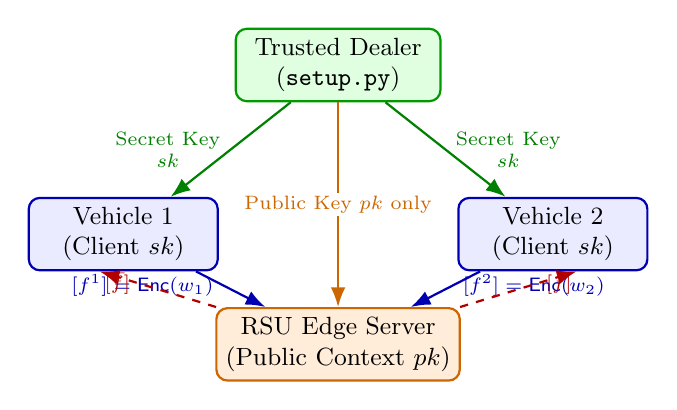
\begin{tikzpicture}[
  node distance = 0.7cm and 0.8cm,
  box/.style   = {draw=blue!70!black, rounded corners=4pt, fill=blue!8,
                  minimum width=2.4cm, minimum height=0.75cm,
                  font=\small, align=center, thick},
  serverbox/.style = {draw=orange!80!black, rounded corners=4pt, fill=orange!15,
                  minimum width=2.6cm, minimum height=0.8cm,
                  font=\small, align=center, thick},
  dealerbox/.style = {draw=green!60!black, rounded corners=4pt, fill=green!12,
                  minimum width=2.6cm, minimum height=0.75cm,
                  font=\small, align=center, thick},
  arrow/.style  = {-{Latex[length=2.5mm]}, thick},
  dasharrow/.style = {-{Latex[length=2.5mm]}, thick, dashed}
]

%% Nodes
\node[dealerbox] (td)  {Trusted Dealer\\(\texttt{setup.py})};
\node[box, below left=1.2cm and 0.2cm of td]  (c1) {Vehicle 1\\(Client $sk$)};
\node[box, below right=1.2cm and 0.2cm of td] (c2) {Vehicle 2\\(Client $sk$)};
\node[serverbox, below=2.6cm of td] (srv) {RSU Edge Server\\(Public Context $pk$)};

%% Key Distribution
\draw[arrow, green!50!black] (td) -- node[left, font=\scriptsize, align=center] {Secret Key\\$sk$} (c1);
\draw[arrow, green!50!black] (td) -- node[right, font=\scriptsize, align=center] {Secret Key\\$sk$} (c2);
\draw[arrow, orange!80!black] (td) -- node[fill=white, font=\scriptsize, inner sep=1pt] {Public Key $pk$ only} (srv);

%% Upload
\draw[arrow, blue!70!black] (c1) -- node[left, font=\scriptsize, pos=0.4] {$[f^1] = \mathsf{Enc}(w_1)$} (srv);
\draw[arrow, blue!70!black] (c2) -- node[right, font=\scriptsize, pos=0.4] {$[f^2] = \mathsf{Enc}(w_2)$} (srv);

%% Downlink
\draw[dasharrow, red!70!black] (srv) -- node[left, font=\scriptsize, pos=0.65] {$[\bar{f}]$} ([xshift=-3mm]c1.south);
\draw[dasharrow, red!70!black] (srv) -- node[right, font=\scriptsize, pos=0.65] {$[\bar{f}]$} ([xshift=3mm]c2.south);

\end{tikzpicture}
\caption{Proposed Single-Key CKKS Federated IoV Architecture. The Trusted Dealer issues the private context containing secret key $sk$ exclusively to vehicle clients. The RSU server receives only the public evaluation context $pk$, guaranteeing mathematical blindness during federated aggregation.}
\label{fig:arch}
\end{figure}

The architecture comprises three operational roles (Fig.~\ref{fig:arch}):

\subsection{Trusted Dealer}
Prior to federated execution, an offline trusted dealer initializes the CKKS
cryptographic context:
\begin{equation}
  \mathsf{ctx} \leftarrow \mathsf{CKKS.Setup}(N=8192, \mathbf{q}, \Delta=2^{40})
\end{equation}
The secret key is serialized as \texttt{secret\_context.bin} for vehicle
clients. Crucially, the dealer executes \texttt{context.make\_context\_public()}
to permanently erase the secret key from memory before generating
\texttt{public\_context.bin} for the RSU server.

\subsection{Removal of AES Transport Security}
In our preliminary Generation-1 design, the V2X transport layer utilized an ECDH
key exchange and AES-256-GCM symmetric encryption. In the current Generation-2
architecture, we deliberately removed this symmetric transport security layer.
Because the CKKS scheme inherently provides payload confidentiality (the RSU
receives only mathematically secure ciphertexts), the additional AES encryption
and TLS handshakes were deemed redundant for confidentiality. This removal streamlines V2X communications and minimizes latency.

\section{Conclusion}
This paper presented a robust Single-Key CKKS Homomorphic Encryption approach 
coupled with a ChebyshevKAN architecture for intrusion detection in IoV. 
By delegating the secret key only to the vehicle nodes and providing a public 
evaluation key to the RSU, the system successfully eliminates the privacy dilemma 
of standard federated learning. In our design, all payload confidentiality is strictly handled 
by CKKS, removing the overhead of traditional transport security mechanisms (such as AES). 
The results indicate excellent detection accuracy across various IoV datasets while maintaining complete mathematical blindness at the aggregation server.

\end{document}
